\documentclass[titlepage,12pt]{article}
\usepackage[utf8]{inputenc}
\usepackage[spanish]{babel}
\usepackage{parskip}
\usepackage[margin= 2.5cm]{geometry}
\usepackage{graphicx}
\usepackage{float}
\usepackage{subcaption}

\title{\textbf{Práctica 2 \\ Teoría de Autómatas y lenguajes formales}}
\author{Jaime Garfia Aragón}
\date{Octubre 2022}

\begin{document}

\maketitle

\section*{\textbf{\underline{Introducción}}}
En esta práctica aprendemos a utilizar ubuntu bajo el uso de la máquina virtual, aprendemos a utilizar GNU octave y hacemos una introducción a \LaTeX.

\section*{\textbf{}{Actividades:}}

\begin{enumerate}
        \item Find the power set $R^3
of R$ = \{(1, 1),(1, 2),(2, 3),(3, 4)\}. Check your answer with the script \textbf{powerrelation.m} and write a   \LaTeX \ document with the
solution step by step.
    
    \item Within the folder “files”, find a TEX file in whose content appears the string \\
\textbf{/usepackage\{amsthm, amsmath\}}. Note: use \textbf{grep} and escape the special
characters with /. Complete the proof and answer the question.

\newpage
\section*{Realizacion actividades}
\textbf{Actividad 1:}

\begin{figure}[h]
    \centering
    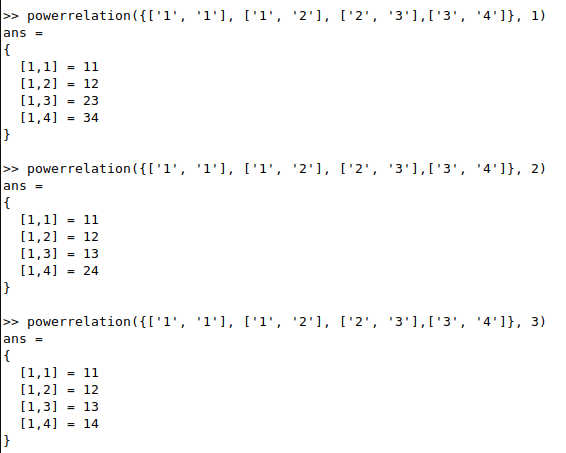
\includegraphics[width=0.8\textwidth]{Powerrelation.png}
    \caption{Potencia de $R^3
of R$ = \{(1, 1),(1, 2),(2, 3),(3, 4)\}}
    \label{fig:fig1}
\end{figure}
Como podemos observar en la imagen \ref{fig:fig1} vamos a realizar paso por paso las potencias de $R$, empezando por $R^2$ y finalmente $R^3$.

\textbf{Actividad 2:}
Consideremos $L=\{w\in \{a,b\}^* : w \textnormal{ no termina en } ab\}$. Un expresión regular que genera L es: \\
$(a+b)^* ba $


\end{enumerate}

\end{document}
